%\iffalse
\let\negmedspace\undefined
\let\negthickspace\undefined

\documentclass[journal,12pt,onecolumn]{IEEEtran}

\usepackage{cite}
\usepackage{amsmath,amssymb,amsfonts,amsthm}
\usepackage{graphicx}
\usepackage{textcomp}
\usepackage{xcolor}
\usepackage{txfonts}
\usepackage{listings}
\usepackage{enumitem}
\usepackage{mathtools}
\usepackage{gensymb}
\usepackage[breaklinks=true]{hyperref}
\usepackage{tkz-euclide}
\usepackage{listings}
\usepackage{float}

\newtheorem{theorem}{Theorem}[section]
\newtheorem{problem}{Problem}
\newtheorem{proposition}{Proposition}[section]
\newtheorem{lemma}{Lemma}[section]
\newtheorem{corollary}[theorem]{Corollary}
\newtheorem{example}{Example}[section]
\newtheorem{definition}[problem]{Definition}
\newcommand{\BEQA}{\begin{eqnarray}}
\newcommand{\EEQA}{\end{eqnarray}}
\newcommand{\define}{\stackrel{\triangle}{=}}
\theoremstyle{remark}
\newtheorem{rem}{Remark}

\begin{document}

\providecommand{\pr}[1]{\ensuremath{\Pr\left(#1\right)}}
\providecommand{\prt}[2]{\ensuremath{p_{#1}^{\left(#2\right)} }}
\providecommand{\qfunc}[1]{\ensuremath{Q\left(#1\right)}}
\providecommand{\sbrak}[1]{\ensuremath{{}\left[#1\right]}}
\providecommand{\lsbrak}[1]{\ensuremath{{}\left[#1\right.}}
\providecommand{\rsbrak}[1]{\ensuremath{{}\left.#1\right]}}
\providecommand{\brak}[1]{\ensuremath{\left(#1\right)}}
\providecommand{\lbrak}[1]{\ensuremath{\left(#1\right.}}
\providecommand{\rbrak}[1]{\ensuremath{\left.#1\right)}}
\providecommand{\cbrak}[1]{\ensuremath{\left\{#1\right\}}}
\providecommand{\lcbrak}[1]{\ensuremath{\left\{#1\right.}}
\providecommand{\rcbrak}[1]{\ensuremath{\left.#1\right\}}}
\newcommand{\sgn}{\mathop{\mathrm{sgn}}}
\providecommand{\abs}[1]{\left\vert#1\right\vert}
\providecommand{\res}[1]{\Res\displaylimits_{#1}} 
\providecommand{\norm}[1]{\left\lVert#1\right\rVert}
\providecommand{\mtx}[1]{\mathbf{#1}}
\providecommand{\mean}[1]{E\left[ #1 \right]}
\providecommand{\cond}[2]{#1\middle|#2}
\providecommand{\fourier}{\overset{\mathcal{F}}{ \rightleftharpoons}}
\newenvironment{amatrix}[1]{%
  \left(\begin{array}{@{}*{#1}{c}|c@{}}
}{%
  \end{array}\right)
}
\newcommand{\solution}{\noindent \textbf{Solution: }}
\newcommand{\cosec}{\,\text{cosec}\,}
\providecommand{\dec}[2]{\ensuremath{\overset{#1}{\underset{#2}{\gtrless}}}}
\newcommand{\myvec}[1]{\ensuremath{\begin{pmatrix}#1\end{pmatrix}}}
\newcommand{\mydet}[1]{\ensuremath{\begin{vmatrix}#1\end{vmatrix}}}
\newcommand{\myaugvec}[2]{\ensuremath{\begin{amatrix}{#1}#2\end{amatrix}}}
\providecommand{\rank}{\text{rank}}
\providecommand{\pr}[1]{\ensuremath{\Pr\left(#1\right)}}
\providecommand{\qfunc}[1]{\ensuremath{Q\left(#1\right)}}
	\newcommand*{\permcomb}[4][0mu]{{{}^{#3}\mkern#1#2_{#4}}}
\newcommand*{\perm}[1][-3mu]{\permcomb[#1]{P}}
\newcommand*{\comb}[1][-1mu]{\permcomb[#1]{C}}
\providecommand{\qfunc}[1]{\ensuremath{Q\left(#1\right)}}
\providecommand{\gauss}[2]{\mathcal{N}\ensuremath{\left(#1,#2\right)}}
\providecommand{\diff}[2]{\ensuremath{\frac{d{#1}}{d{#2}}}}
\providecommand{\myceil}[1]{\left \lceil #1 \right \rceil }
\newcommand\figref{Fig.~\ref}
\newcommand\tabref{Table~\ref}
\newcommand{\sinc}{\,\text{sinc}\,}
\newcommand{\rect}{\,\text{rect}\,}
\let\vec\mathbf
\bibliographystyle{IEEEtran}
\bigskip
Q: Consider the wave elevation spectrum $S_{\eta \eta}(\omega)$ as shown in the figure. Then, the significant wave height is \underline{\hspace{3cm}} m.
\begin{figure}[H]
    \centering
    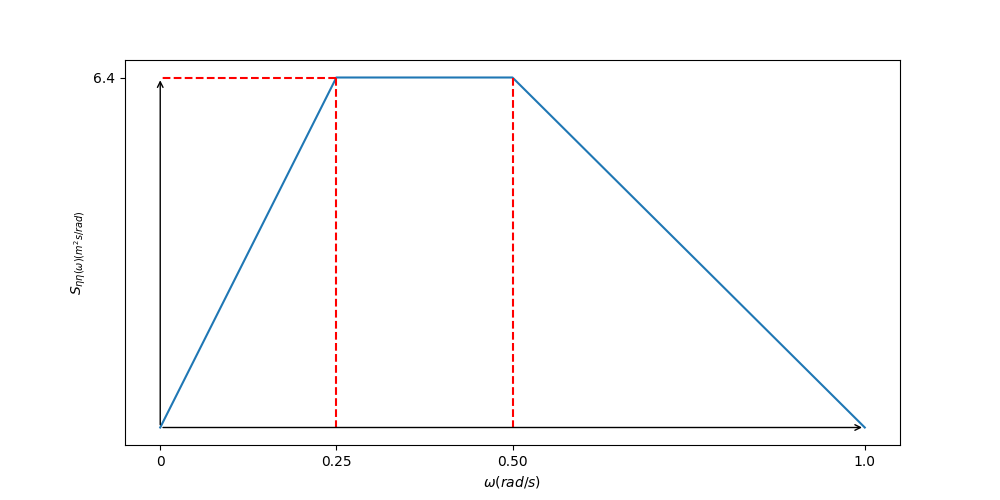
\includegraphics[width=\columnwidth]{./figs/qfig.png}
    \caption{Wave Elevation Spectrum}
    \label{fig: GATE22NM40.1}
\end{figure}

\begin{enumerate}[label=(\Alph*)]
\item 2
\item 4
\item 6
\item 8
\end{enumerate}
\hfill{GATE NM 2022}


\solution
%\fi
Given:
\begin{align}
S_{\eta \eta}(\omega)(m^2s/rad) = 
\begin{cases}
  25.6\omega   & \text{if } \omega \in [0,0.25] \\
  6.4  & \text{if } \omega \in (0.25,0.50] \\
  12.8\omega-12.8  & \text{if } \omega \in (0.50,1.0] \\
  0  & o.w \\
\end{cases}
\end{align}
In terms of f:
\begin{align}
S_{\eta \eta}(f)(m^2s) = 
\begin{cases}
  51.2\pi f   & \text{if } f \in [0,\frac{\pi}{2}] \\
  6.4  & \text{if } f \in (\frac{\pi}{2},\pi] \\
  25.6\pi f-12.8  & \text{if } f \in (\pi,2\pi] \\
  0 & o.w \\
\end{cases} \label{eq: GATE22NM40.1}
\end{align}
Significant Wave Height:
\begin{align}
H_s &= 4 \sqrt{\int_{0}^{\infty} S(f)df}
\end{align}
From \eqref{eq: GATE22NM40.1}
\begin{align}
H_s &= 4 \sqrt{\int_{0}^{\frac{\pi}{2}} 51.2\pi fdf + \int_{\frac{\pi}{2}}^{\pi} 6.4df + \int_{\pi}^{2\pi} (25.6\pi f-12.8)df} \\
&= 4 \sqrt{0.8 +1.6 +1.6} \\
\therefore H_s &= 4
\end{align}
Hence the answer is option (D).
%table
%\begin{table}[!h]
%\begin{tabular}{|c|c|c|} 
      \hline
\textbf{Variable}& \textbf{Description}& \textbf{Value}\\\hline
	 $H(z)$ & Transfer Function & $\beta_0z^{-1} + \beta_1$ \\\hline
         $\abs{H(z)}_{max}$ & Maximum value of Transfer Function & 1 \\\hline  
         $\abs{H(z)}_{min}$ & Minimum value of Transfer Function & $\frac{1}{2}$\\\hline
    \end{tabular}

%\caption{Input Parameter Table}
%\label{tab:q.no.1}
%\end{table}

%figure
%\begin{figure}[H]
%    \centering
%    \includegraphics[width=\columnwidth]{./figs/fig.png}
%    \caption{caption}
%    \label{fig: q.no.1}
%\end{figure}

\end{document}
